\documentclass[xcolor=dvipsnames, aspectratio=1610]{beamer}

\usepackage{fontspec}
\usepackage{xeCJK}

% Beamer mặc định là sans-serif → giữ nguyên
\renewcommand{\familydefault}{\sfdefault}
\setsansfont{Latin Modern Sans}  % hoặc không cần nếu để mặc định Beamer

% Font CJK có sẵn (Windows/macOS)
\setCJKmainfont{MS Gothic}       % hoặc Meiryo / Yu Gothic / Hiragino Sans

% Các gói phụ khác
\usepackage{minibox}
\usepackage{color}
\usepackage{lipsum}
\usepackage{hyperref}
\usepackage{tikz}
\usepackage{listings}
\usepackage{multicol}
\usepackage{multirow}
\usepackage{amsmath}
\usepackage{forest}
\usepackage[table]{xcolor}
\usepackage{graphicx}
\usepackage{algorithm}
\usepackage{caption}

\definecolor{CutePink}{RGB}{255, 102, 178}
\usetheme{Ilmenau}
\usecolortheme[named=CutePink]{structure}

\title[インターネットによる詐欺・その防止対策]{\Huge インターネットによる詐欺・その防止対策}
\subtitle{\large 日本語8の最終発表}
\author[グループ2 - C2]{\LARGE \textbf{グループ2 - C2}}
\institute[日本語8]{\Large 日本語8}
\date[\today]{\large ハノイ工科大学、2025年06月15日}

% Thiết lập background cho toàn bộ slide
\setbeamertemplate{background}{
    \begin{tikzpicture}[remember picture,overlay]
        \node[opacity=0.25, at=(current page.center)] {
        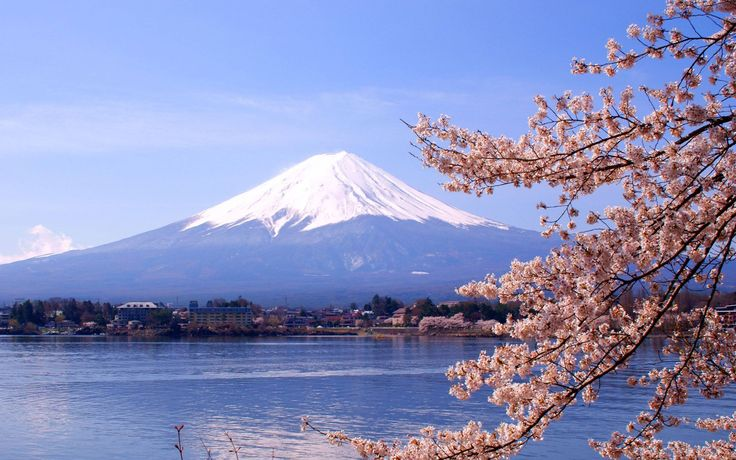
\includegraphics[width=\paperwidth,height=\paperheight]{images/background.jpg}
        };
    \end{tikzpicture}
}


\begin{document}

\begin{frame}
\maketitle
\end{frame}

\begin{frame}{グループ2のメンバー}
    \LARGE
    \begin{itemize}
        \item \textbf{ドー・ザ・フイ - 20215060}
        \item \textbf{ドー・ヴァン・ビン - 20210103}
        \item \textbf{グエン・ゴック・キエン - 20215069}
        \item \textbf{グイ・カック・フィ・ロン - 20210966}
    \end{itemize}
\end{frame}

\begin{frame}{目次}
    \tableofcontents
\end{frame}

\section{はじめに}
\begin{frame}{目次}
    \tableofcontents[currentsection, hideothersubsections] 
\end{frame}
\begin{frame}{テーマのご紹介}
    インターネットはとても便利ですが、危険もあります。その中で、詐欺がとてもふえています。
    \vspace{0.3cm}
    \begin{figure}[h]
        \centering
        \raisebox{1cm}{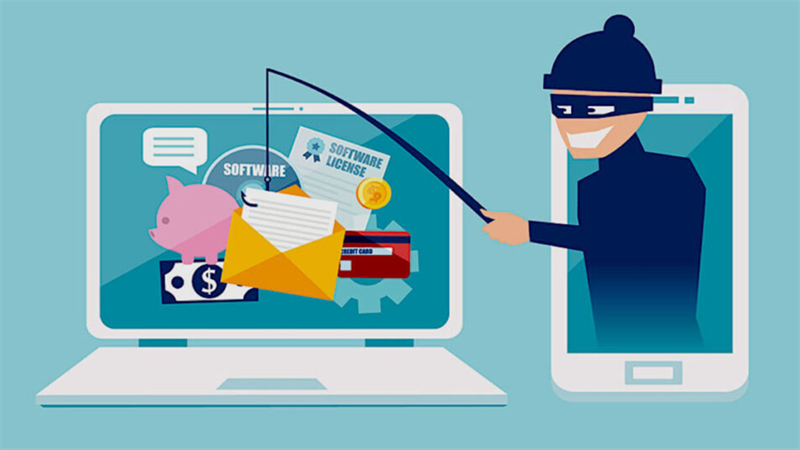
\includegraphics[width=0.65\textwidth]{images/1.png}}
    \end{figure}
\end{frame}

\section{インターネット詐欺の現状と具体例}
\begin{frame}{目次}
    \tableofcontents[currentsection, hideothersubsections] 
\end{frame}
\begin{frame}{現状}
    \LARGE
    \textbf{今は、インターネット詐欺は世界中で起きています。} \\
    \pause
    \textbf{\alert{もちろん、ベトナムや日本でも増えています。}}
\end{frame}
\begin{frame}[t]{よくある詐欺の手口}
    \textbf{よくある詐欺の手口の例:}
    \begin{columns}
        \begin{column}{0.5\textwidth}
            \begin{figure}[h]
                \centering
                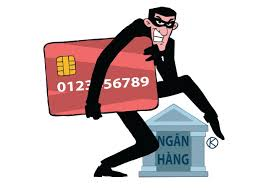
\includegraphics[width=0.8\textwidth]{images/2.jpg}
            \end{figure}
        \end{column}
        \begin{column}{0.5\textwidth}
            \begin{figure}[h]
                \centering
                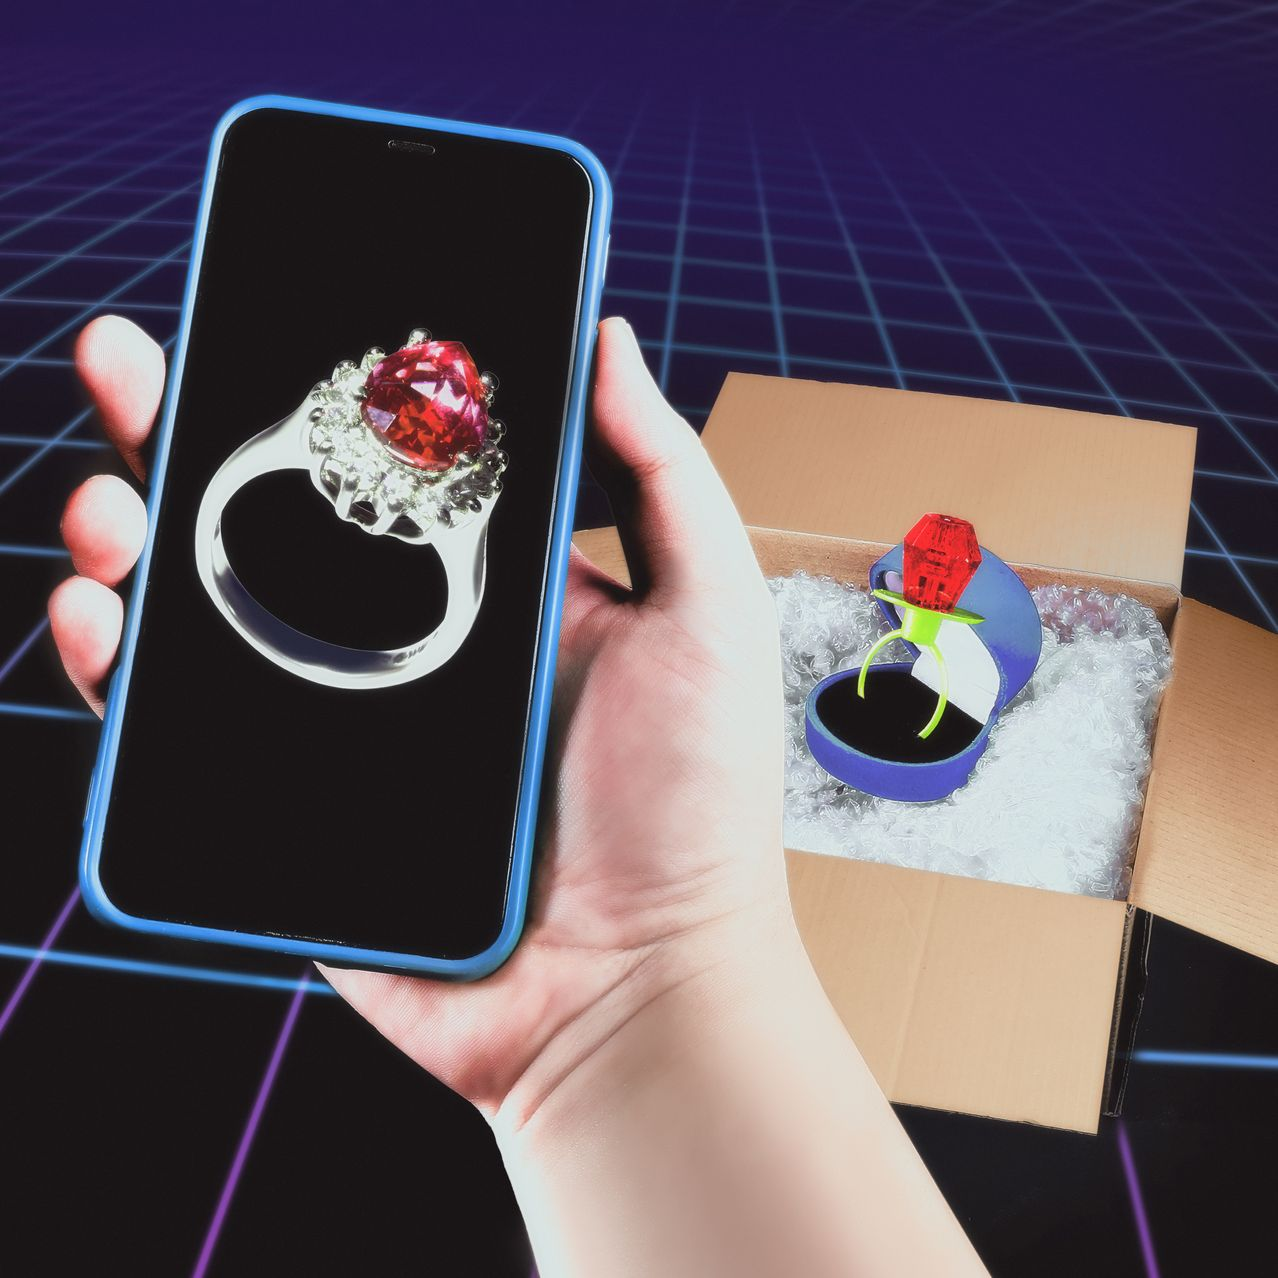
\includegraphics[width=0.8\textwidth]{images/3.jpeg}
            \end{figure}
        \end{column}
    \end{columns}
\end{frame}
\begin{frame}{結論}
    \LARGE
    \textbf{このような問題は増えていて、見分けるのが難しいです。} \\
    \vspace{0.5cm}
    \textbf{\alert{$\Rightarrow$ 特に、高齢者やネットが苦手な人はあぶないです。}}
\end{frame}

\section{防止方法}
\begin{frame}{目次}
    \tableofcontents[currentsection, hideothersubsections] 
\end{frame}
\begin{frame}{1. パスワードや情報を他人に教えない。}
    \begin{figure}[h]
        \centering
        \raisebox{1cm}{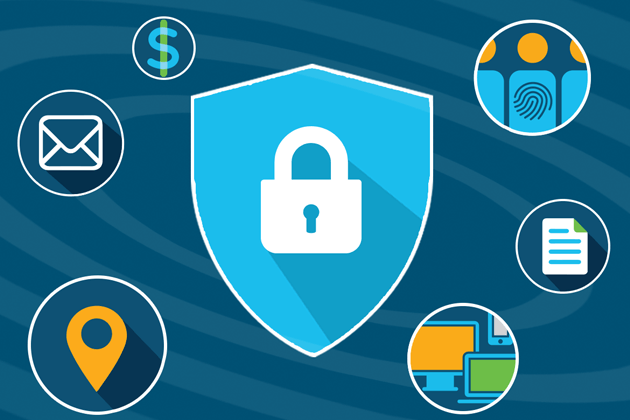
\includegraphics[width=0.65\textwidth]{images/41.png}}
    \end{figure}
\end{frame}
\begin{frame}{2. ログイン前に、サイトのアドレスを確認する。}
    \begin{figure}[h]
        \centering
        \raisebox{1cm}{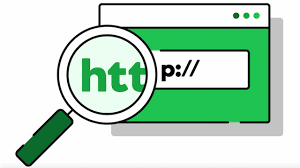
\includegraphics[width=0.65\textwidth]{images/42.png}}
    \end{figure}
\end{frame}
\begin{frame}{3. 「お金がすぐにもうかる」などの話をしんじない。}
    \begin{figure}[h]
        \centering
        \raisebox{1cm}{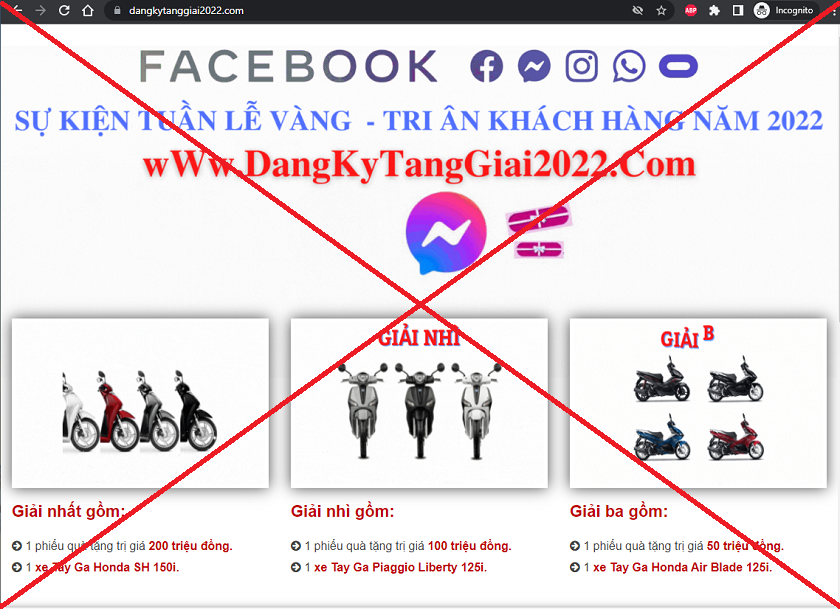
\includegraphics[width=0.65\textwidth]{images/43.png}}
    \end{figure}
\end{frame}
\begin{frame}{4. ウイルス対策ソフトを使う。}
    \begin{figure}[h]
        \centering
        \raisebox{1cm}{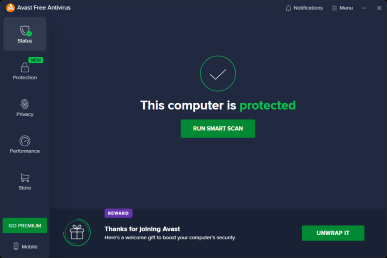
\includegraphics[width=0.65\textwidth]{images/44.png}}
    \end{figure}
\end{frame}
\begin{frame}{5. あやしい時は、家族、先生、警察に相談する。}
    \begin{figure}[h]
        \centering
        \raisebox{1cm}{
\includegraphics[width=0.65\textwidth]{images/45.jpg}}
    \end{figure}
\end{frame}

\section{まとめ}
\begin{frame}{目次}
    \tableofcontents[currentsection, hideothersubsections] 
\end{frame}
\begin{frame}{まとめ}
    \begin{figure}[h]
        \centering
        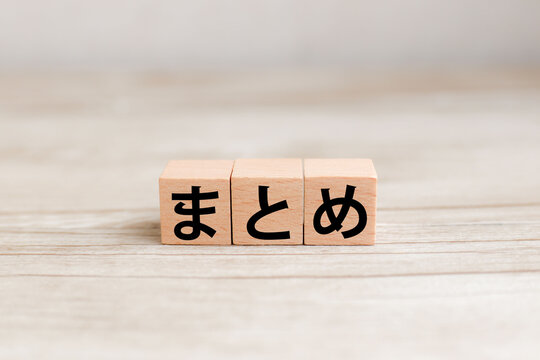
\includegraphics[height=0.65\textheight]{images/5.jpg}
    \end{figure}
    \textbf{$\Rightarrow$ インターネットは便利ですが、注意も必要です。だまされないように、よく考えてから行動しましょう。}
\end{frame}

\section*{}
{
\setbeamertemplate{headline}{} % Tạm thời ẩn thanh đầu trong slide này
\begin{frame}{Q\&A}
    \begin{figure}[h]
        \centering
        
\includegraphics[height=0.85\textheight]{images/6.jpg}
    \end{figure}
\end{frame}
}

\end{document}
